\documentclass[aspectratio=169]{beamer}

% VT presentation template (Overleaf: pncrbgxvdjzj)
\usetheme{Madrid}
\useoutertheme{miniframes}
\useinnertheme{circles}

\usepackage[utf8]{inputenc}
\usepackage[T1]{fontenc}
\usepackage{palatino}
\usepackage[default]{opensans}
\usefonttheme{default}

\usepackage{graphicx}
\usepackage{booktabs}
\usepackage{amsmath}
\usepackage{tikz}
\usepackage{colortbl}

\usetikzlibrary{positioning, arrows.meta, shapes.geometric, calc}

% Speaker notes toggle
\ifdefined\SHOWNOTES
  \usepackage{pgfpages}
  \setbeameroption{show notes on second screen=right}
\fi

% Virginia Tech official colors (VT template)
\definecolor{myRed}{RGB}{134,31,65}       % VT Maroon
\definecolor{myOrange}{RGB}{229,117,31}   % VT Orange
% Legacy aliases kept so existing TikZ frames keep working
\colorlet{vtMaroon}{myRed}
\colorlet{vtOrange}{myOrange}
\colorlet{mTeal}{myRed}
\colorlet{mBrown}{myOrange}
\definecolor{mRed}{HTML}{CC4444}     % error/warning
\definecolor{mGreen}{HTML}{4A9A4A}   % success/done
\definecolor{mGray}{HTML}{888888}    % neutral

% VT template color assignments
\setbeamercolor{frametitle}{bg=myRed!85, fg=white}
\setbeamercolor{title}{fg=white, bg=myRed}
\setbeamercolor{subtitle}{fg=white}
\setbeamercolor{author}{fg=myRed}
\setbeamercolor{institute}{fg=myRed}
\setbeamercolor{date}{fg=myRed}
\setbeamercolor{structure}{fg=myRed}
\setbeamercolor{itemize item}{fg=myOrange}
\setbeamercolor{itemize subitem}{fg=myOrange}
\setbeamercolor{enumerate item}{fg=myOrange}
\setbeamercolor{section in head/foot}{bg=myRed, fg=white}
\setbeamercolor{subsection in head/foot}{bg=myRed!80, fg=white}
\setbeamercolor{section in toc}{fg=myRed}
\setbeamercolor{alerted text}{fg=myOrange}
\setbeamercolor{block title}{bg=myOrange!80, fg=white}
\setbeamercolor{block body}{bg=myOrange!10}

% VT monogram command (TikZ vector logo; used in institute line)
\newcommand{\vtlogo}[1][0.8cm]{%
  
\begin{tikzpicture}[baseline=(V.base)]
    \node[font=\bfseries\fontsize{16}{16}\selectfont, text=myRed, inner sep=0pt] (V) {V};
    \node[font=\bfseries\fontsize{16}{16}\selectfont, text=myOrange, inner sep=0pt, anchor=west] at ([xshift=-1pt]V.east) {T};
  \end{tikzpicture}%
}

\title{CHIME}
\subtitle{A Cache-Efficient and High-Performance Hybrid Index\\on Disaggregated Memory}
\author{Jason Cusati}
\institute[VT CS]{CS 6204 --- Advanced Topics in Systems\\Virginia Tech}
\date{April 9, 2026}

% VT logo bottom-right on every slide
\logo{\vtlogo}

\begin{document}

% ============================================================
% SECTION 1: What is CHIME? (5 slides, ~3 min)
% ============================================================

% Slide 1 — Title
\maketitle
\note{
  \textbf{Key point:} Introduction.\\
  \textbf{Say:} Good morning, I'm Jason Cusati, presenting my progress
  on reproducing CHIME for CS 6204.\\
  \textbf{Transition:} Let's start with the problem CHIME solves.\\
  \textbf{Time:} 15s
}

% Slide 2 — The Problem
\begin{frame}{Disaggregated Memory Indexes}
\centering
\includegraphics[height=0.82\textheight]{diagrams/tradeoff.pdf}
\note{
  \textbf{Key point:} DM range indexes face a cache vs read-amp trade-off.\\
  \textbf{Say:} Disaggregated memory separates compute and memory over
  a network. Range indexes on DM face a fundamental trade-off: B+ trees
  cache well but need multiple round trips per lookup, while hash indexes
  are fast but consume huge cache. CHIME breaks this trade-off.\\
  \textbf{Transition:} Here's how CHIME does it.\\
  \textbf{Time:} 45s
}
\end{frame}

% Slide 3 — The Insight
\begin{frame}{CHIME: Hybrid Structure}
\centering
\includegraphics[height=0.82\textheight]{diagrams/hybrid-structure.pdf}
\note{
  \textbf{Key point:} Hybrid = tree structure + hash leaves.\\
  \textbf{Say:} CHIME keeps B+ tree internal nodes for structure
  and range query support, but replaces sorted leaves with
  hopscotch hashing. Internal nodes cache well because there
  are few of them. Leaves use hashing to find keys in one
  round trip instead of binary search.\\
  \textbf{Transition:} Three specific techniques make this work.\\
  \textbf{Time:} 45s
}
\end{frame}

% Slide 4 — Three Techniques
\begin{frame}{Three Key Techniques}
\centering
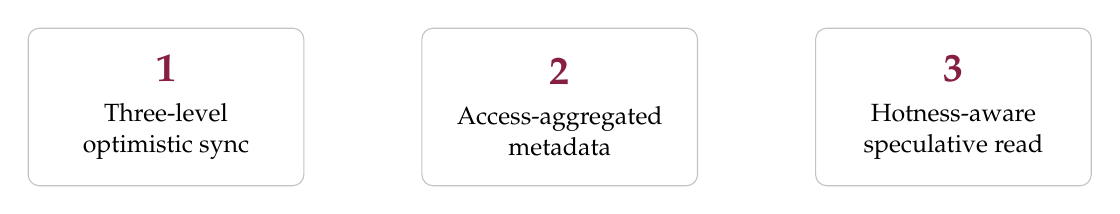
\begin{tikzpicture}[
  card/.style={draw=mGray!50, rounded corners=4pt, minimum width=3.5cm,
               minimum height=2cm, align=center, font=\small},
]
  \node[card] (t1) at (-5,0) {
    {\Large\color{mTeal} \textbf{1}}\\[0.4em]
    Three-level\\optimistic sync
  };
  \node[card] (t2) at (0,0) {
    {\Large\color{mTeal} \textbf{2}}\\[0.4em]
    Access-aggregated\\metadata
  };
  \node[card] (t3) at (5,0) {
    {\Large\color{mTeal} \textbf{3}}\\[0.4em]
    Hotness-aware\\speculative read
  };
\end{tikzpicture}
\note{
  \textbf{Key point:} Three techniques enable the hybrid design.\\
  \textbf{Say:} Three techniques make this work. First, three-level
  optimistic synchronization reuses hopscotch bitmaps for fine-grained
  concurrency---no global locks. Second, vacancy bitmap piggybacking
  and metadata replication reduce round trips for metadata. Third,
  a hotspot buffer shortcuts reads for frequently accessed neighborhoods.\\
  \textbf{Transition:} What does this achieve?\\
  \textbf{Time:} 50s
}
\end{frame}

% Slide 5 — The Claim
{
\setbeamercolor{background canvas}{bg=myRed}
\begin{frame}[plain]
\vspace*{\fill}
\begin{center}
{\color{white}\Huge\bfseries Up to 5.1\texttimes{} throughput}\\[0.6em]
{\color{white}\Huge\bfseries 8.7\texttimes{} less cache}
\end{center}
\vspace*{\fill}
\note{
  \textbf{Key point:} CHIME's headline result.\\
  \textbf{Say:} The paper's headline: up to 5.1 times higher throughput
  than SMART with the same cache size, or similar performance with
  8.7 times less cache. Strong numbers---but we should examine
  how they were earned.\\
  \textbf{Transition:} Before the experiments, let's look at the
  strengths and weaknesses of the paper itself.\\
  \textbf{Time:} 30s
}
\end{frame}
}

% ============================================================
% SECTION 2: Strengths & Weaknesses (3 slides, ~3 min)
% ============================================================

\section{Strengths \& Weaknesses}

% Slide 6 — Strengths
\begin{frame}{Strengths}
\centering
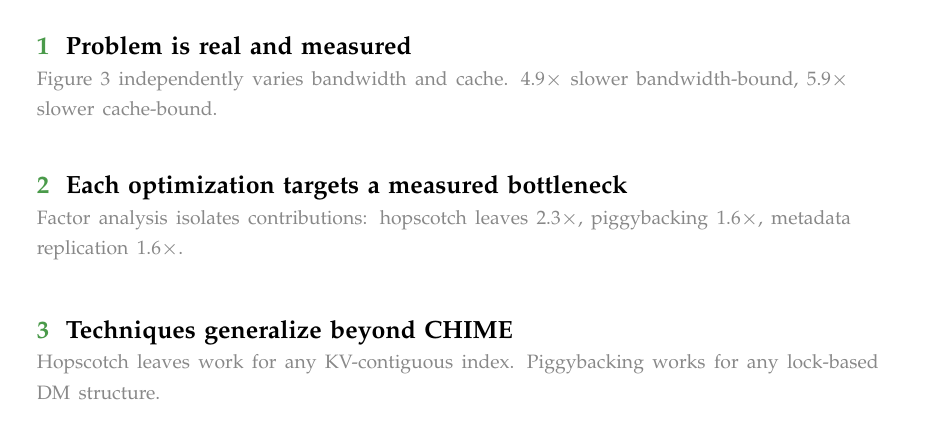
\begin{tikzpicture}[
  item/.style={font=\small, anchor=west, align=left, text width=11cm},
]
  \node[item] at (-5.5, 1.8)
    {{\color{mGreen}\textbf{1}}~~\textbf{Problem is real and measured}\\
     {\color{mGray}\scriptsize Figure 3 independently varies bandwidth and cache.
                              4.9$\times$ slower bandwidth-bound, 5.9$\times$ slower cache-bound.}};
  \node[item] at (-5.5, 0)
    {{\color{mGreen}\textbf{2}}~~\textbf{Each optimization targets a measured bottleneck}\\
     {\color{mGray}\scriptsize Factor analysis isolates contributions: hopscotch leaves 2.3$\times$,
                              piggybacking 1.6$\times$, metadata replication 1.6$\times$.}};
  \node[item] at (-5.5,-1.8)
    {{\color{mGreen}\textbf{3}}~~\textbf{Techniques generalize beyond CHIME}\\
     {\color{mGray}\scriptsize Hopscotch leaves work for any KV-contiguous index.
                              Piggybacking works for any lock-based DM structure.}};
\end{tikzpicture}
\note{
  \textbf{Key point:} Three concrete strengths, each with evidence.\\
  \textbf{Say:} Three things the paper gets right. First, the trade-off
  is not asserted---it's measured. Figure 3 independently varies bandwidth
  and cache and shows 4.9 and 5.9 times slowdowns. Second, each optimization
  targets a measured bottleneck and the factor analysis isolates the
  contribution of each one. Third, the techniques are general---hopscotch
  leaves can apply to any KV-contiguous index and the piggybacking trick
  works for any lock-based DM structure.\\
  \textbf{Transition:} Now the weaknesses.\\
  \textbf{Time:} 50s
}
\end{frame}

% Slide 7 — Weaknesses
\begin{frame}{Weaknesses}
\centering
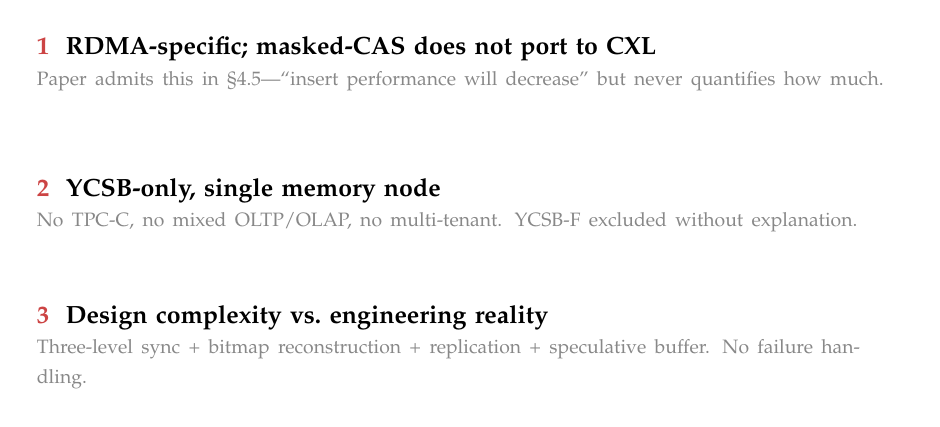
\begin{tikzpicture}[
  item/.style={font=\small, anchor=west, align=left, text width=11cm},
]
  \node[item] at (-5.5, 1.8)
    {{\color{mRed}\textbf{1}}~~\textbf{RDMA-specific; masked-CAS does not port to CXL}\\
     {\color{mGray}\scriptsize Paper admits this in \S4.5---``insert performance will decrease''
                              but never quantifies how much.}};
  \node[item] at (-5.5, 0)
    {{\color{mRed}\textbf{2}}~~\textbf{YCSB-only, single memory node}\\
     {\color{mGray}\scriptsize No TPC-C, no mixed OLTP/OLAP, no multi-tenant. YCSB-F excluded
                              without explanation.}};
  \node[item] at (-5.5,-1.8)
    {{\color{mRed}\textbf{3}}~~\textbf{Design complexity vs.\ engineering reality}\\
     {\color{mGray}\scriptsize Three-level sync + bitmap reconstruction + replication +
                              speculative buffer. No failure handling.}};
\end{tikzpicture}
\note{
  \textbf{Key point:} Three concrete weaknesses, each with evidence.\\
  \textbf{Say:} Three things the paper does not address. One: the most
  impactful optimization---vacancy bitmap piggybacking---depends on
  masked-CAS, which the paper itself admits does not work under CXL.
  No quantification of how much that hurts. Two: evaluation is YCSB only,
  single memory node only, and even YCSB-F is excluded without explanation.
  Three: the design stacks four separate mechanisms and the paper does
  not discuss failure modes, crash consistency, or engineering cost.\\
  \textbf{Transition:} Which raises the question---\\
  \textbf{Time:} 50s
}
\end{frame}

% Slide 8 — The Core Question
{
\setbeamercolor{background canvas}{bg=myRed}
\begin{frame}[plain]
\vspace*{\fill}
\begin{center}
{\color{white}\Huge\bfseries Fundamental breakthrough}\\[0.6em]
{\color{white}\Huge\bfseries or RDMA-era optimization?}
\end{center}
\vspace*{\fill}
\note{
  \textbf{Key point:} The question to hold onto through the rest of the talk.\\
  \textbf{Say:} Is CHIME a fundamental architectural breakthrough, or a
  carefully engineered RDMA-era optimization that will age as the hardware
  landscape shifts? Hold that thought---we'll come back to it in discussion.\\
  \textbf{Transition:} But first, the experiments.\\
  \textbf{Time:} 25s
}
\end{frame}
}

% ============================================================
% SECTION 3: RDMA Experiments + Next Steps (10 slides, ~7 min)
% ============================================================

\section{RDMA Experiments}

% Slide 9 — CloudLab Setup
\begin{frame}{CloudLab Configuration}
\centering
\includegraphics[height=0.82\textheight]{diagrams/cluster-topology.pdf}
\note{
  \textbf{Key point:} Same hardware type as the paper, fewer nodes.\\
  \textbf{Say:} We used CloudLab's r650 nodes at Clemson---same hardware
  family as the paper. Dual 36-core Xeons, 100 Gbps Mellanox ConnectX-6 NIC.
  We had 5 compute nodes plus 1 memory node---half the paper's 10 CN.
  Absolute throughput is lower but relative comparisons are valid.\\
  \textbf{Transition:} Here are the five methods we compared.\\
  \textbf{Time:} 40s
}
\end{frame}

% Slide 10 — Methods Compared
\begin{frame}{Methods Compared}
\centering
\begin{table}
\small
\begin{tabular}{lll}
\toprule
\textbf{Method} & \textbf{Type} & \textbf{Source} \\
\midrule
\rowcolor{mTeal!8}
CHIME & Hybrid (B+ tree + hopscotch) & dmemsys/CHIME \\
Sherman & B+ tree & CHIME repo (diff flags) \\
SMART & Radix tree & dmemsys/SMART \\
ROLEX & Learned index & River861/ROLEX \\
SMART-SC & Radix + sufficient cache & dmemsys/SMART \\
\bottomrule
\end{tabular}
\end{table}
\note{
  \textbf{Key point:} Five methods spanning different index designs.\\
  \textbf{Say:} We compared all five methods from the paper. Sherman is
  a pure B+ tree---actually built from the same CHIME codebase with
  different compile flags. SMART is a radix tree, ROLEX is a learned
  index. SMART-SC is SMART with sufficient cache---the upper bound
  for cache-heavy approaches.\\
  \textbf{Transition:} Honest status check on what we collected.\\
  \textbf{Time:} 40s
}
\end{frame}

% Slide 11 — Experiment Status
\begin{frame}{Experiment Status}
\centering
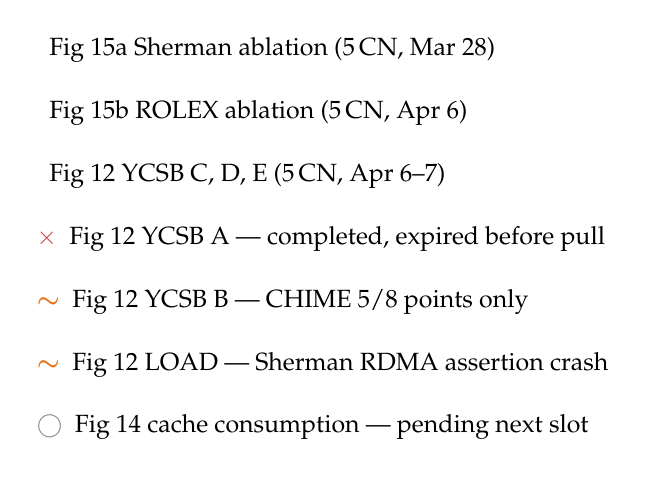
\begin{tikzpicture}[
  item/.style={font=\small, anchor=west},
]
  \node[item] at (0, 2.4) {{\color{mGreen}\checkmark}~~Fig~15a Sherman ablation (5\,CN, Mar 28)};
  \node[item] at (0, 1.6) {{\color{mGreen}\checkmark}~~Fig~15b ROLEX ablation (5\,CN, Apr 6)};
  \node[item] at (0, 0.8) {{\color{mGreen}\checkmark}~~Fig~12 YCSB C, D, E (5\,CN, Apr 6--7)};
  \node[item] at (0, 0.0) {{\color{mRed}$\times$}~~Fig~12 YCSB A --- completed, expired before pull};
  \node[item] at (0,-0.8) {{\color{mBrown}$\boldsymbol{\sim}$}~~Fig~12 YCSB B --- CHIME 5/8 points only};
  \node[item] at (0,-1.6) {{\color{mBrown}$\boldsymbol{\sim}$}~~Fig~12 LOAD --- Sherman RDMA assertion crash};
  \node[item] at (0,-2.4) {{\color{mGray}$\bigcirc$}~~Fig~14 cache consumption --- pending next slot};
\end{tikzpicture}
\note{
  \textbf{Key point:} Honest status: 3 figures done, 3 workloads lost or partial.\\
  \textbf{Say:} Here's what we actually have. Both ablation figures are
  complete. Figure 12 YCSB C, D, and E are complete. But YCSB A finished
  on the memory node and the reservation expired before we could pull
  results. YCSB B is partial---CHIME got 5 of 8 points. YCSB LOAD, Sherman
  crashed with an RDMA assertion. Fig 14 cache consumption is pending
  the next r650 slot.\\
  \textbf{Transition:} Start with what worked.\\
  \textbf{Time:} 50s
}
\end{frame}

% Slide 12 — Ablation Results (fig_15a)
\begin{frame}{Result: Sherman $\to$ CHIME Ablation (r650)}
\centering
\IfFileExists{figures/fig_15a.pdf}{%
  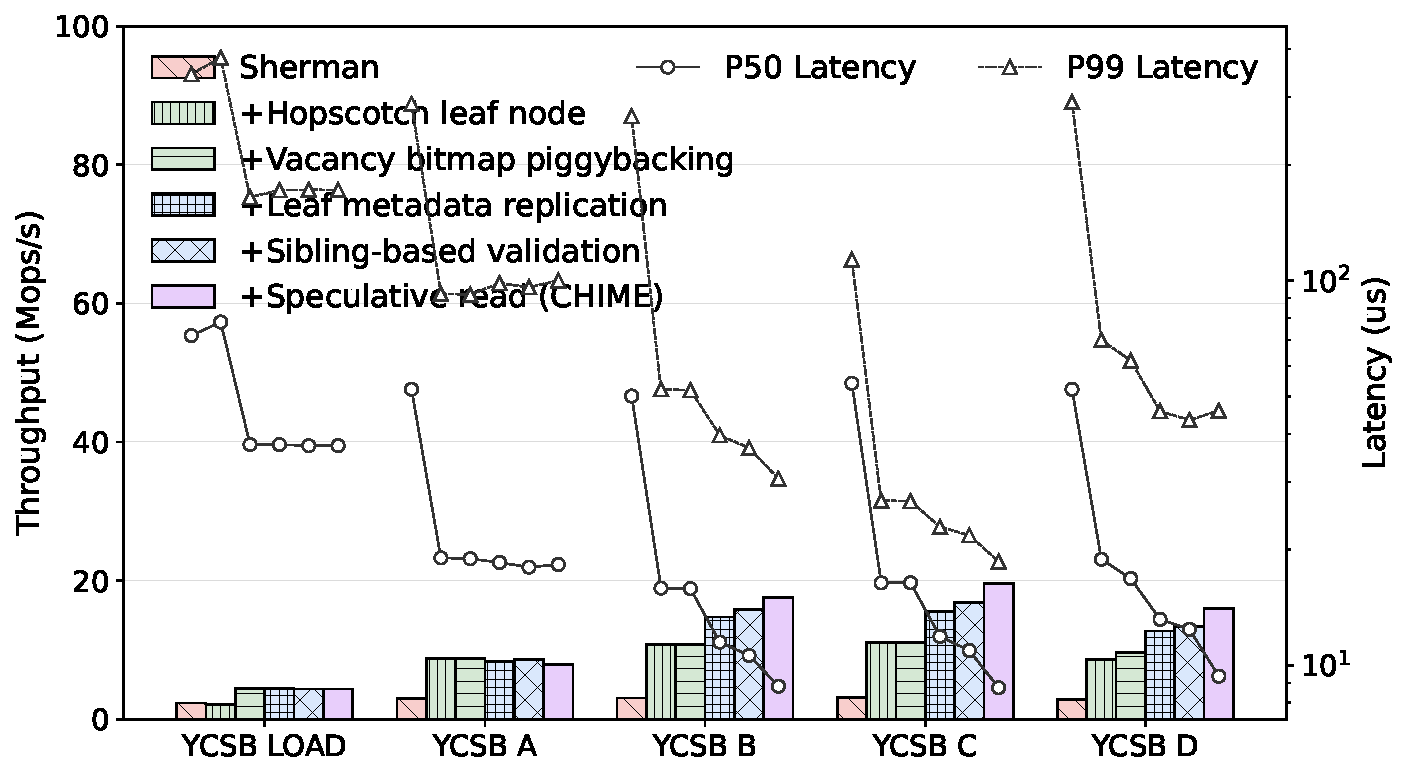
\includegraphics[width=0.95\textwidth]{figures/fig_15a.pdf}%
}{%
  
\includegraphics[width=0.95\textwidth]{../exp/results/fig_15a.pdf}%
}
\note{
  \textbf{Key point:} Each CHIME technique adds measurable throughput.\\
  \textbf{Say:} Here's our r650 data for Fig 15a---the Sherman-to-CHIME
  ablation. Each bar adds one technique. Hopscotch leaves give the biggest
  jump---roughly 3x on reads. Metadata replication adds another chunk on
  read-heavy workloads. Speculative leaf read tops it off for YCSB B and C.
  The pattern matches the paper's claims closely.\\
  \textbf{Transition:} Same pattern against the ROLEX baseline.\\
  \textbf{Time:} 50s
}
\end{frame}

% Slide 13 — Ablation Results (fig_15b)
\begin{frame}{Result: ROLEX $\to$ CHIME Ablation (r650)}
\centering
\IfFileExists{figures/fig_15b.pdf}{%
  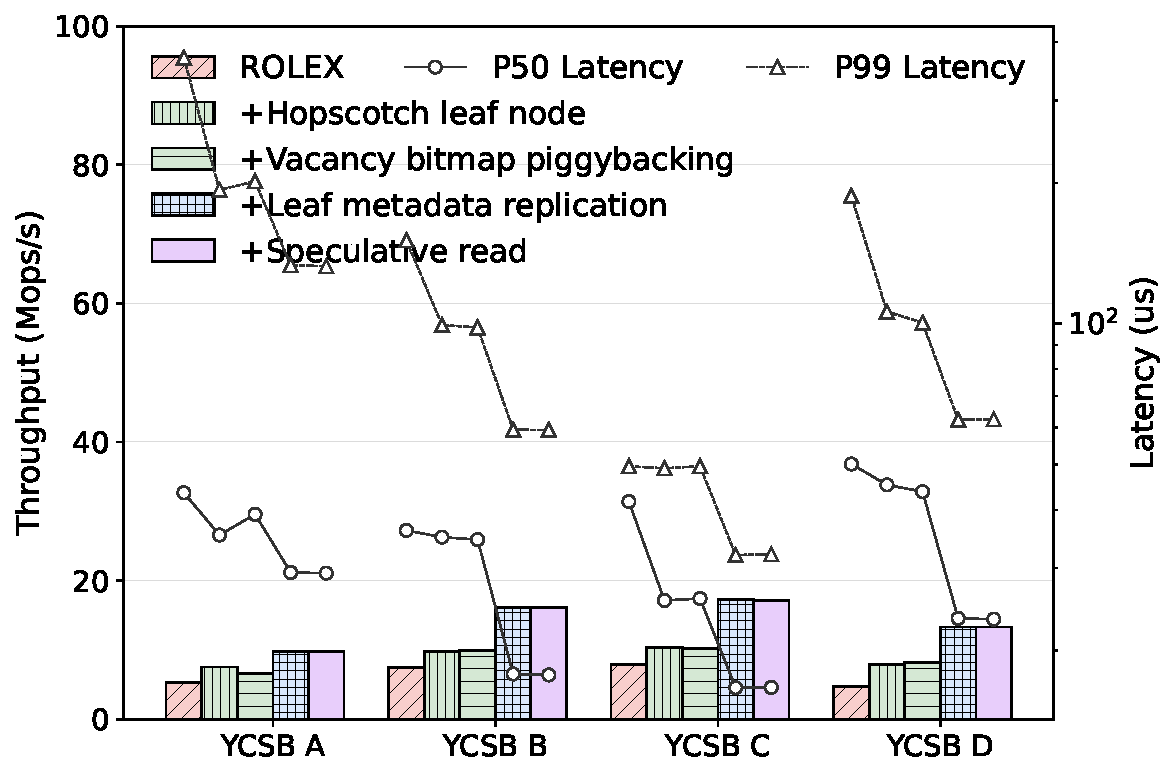
\includegraphics[width=0.95\textwidth]{figures/fig_15b.pdf}%
}{%
  
\includegraphics[width=0.95\textwidth]{../exp/results/fig_15b.pdf}%
}
\note{
  \textbf{Key point:} CHIME techniques also improve the learned index baseline.\\
  \textbf{Say:} Fig 15b starts from ROLEX---the learned index---and adds
  CHIME's techniques incrementally. Metadata replication is the biggest win
  here, nearly doubling throughput on read-heavy workloads. This confirms
  the techniques are general, not specific to the B+ tree baseline.\\
  \textbf{Transition:} And the throughput-latency data.\\
  \textbf{Time:} 45s
}
\end{frame}

% Slide 14 — Throughput-Latency (fig_12_c)
\begin{frame}{Result: Throughput vs Latency --- YCSB C (r650)}
\centering
\IfFileExists{figures/fig_12_c.pdf}{%
  \includegraphics[width=0.9\textwidth]{figures/fig_12_c.pdf}%
}{%
  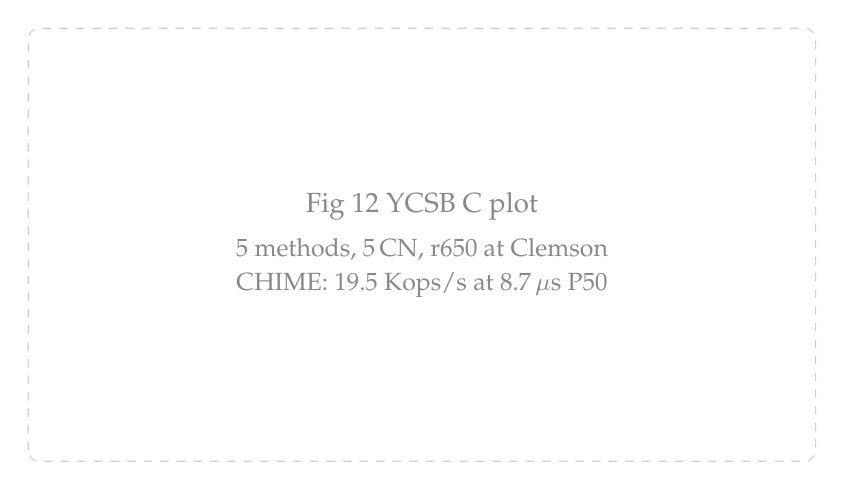
\begin{tikzpicture}
    \draw[mGray!40, dashed, rounded corners=4pt] (0,0) rectangle (10,5.5);
    \node[mGray, align=center, font=\normalsize] at (5,2.75)
      {Fig~12 YCSB~C plot\\[0.4em]
       {\small 5 methods, 5\,CN, r650 at Clemson}\\
       {\small CHIME: 19.5 Kops/s at 8.7\,$\mu$s P50}};
  \end{tikzpicture}%
}
\note{
  \textbf{Key point:} CHIME dominates on read-only workload.\\
  \textbf{Say:} YCSB C is 100\% reads. CHIME reaches 19.5 thousand ops
  per second with only 8.7 microseconds P50 latency---roughly 2.5x Sherman
  and 1.7x ROLEX. The speculative leaf read really shines here because every
  operation benefits from the hotspot buffer. Note we're running 5 compute
  nodes, not the paper's 10, so absolute throughput is lower but the
  relative ordering matches.\\
  \textbf{Transition:} Now what didn't work.\\
  \textbf{Time:} 50s
}
\end{frame}

% Slide 15 — What Failed: The RoCE Rabbit Hole
\begin{frame}{What Failed: The RoCE Rabbit Hole}
\centering
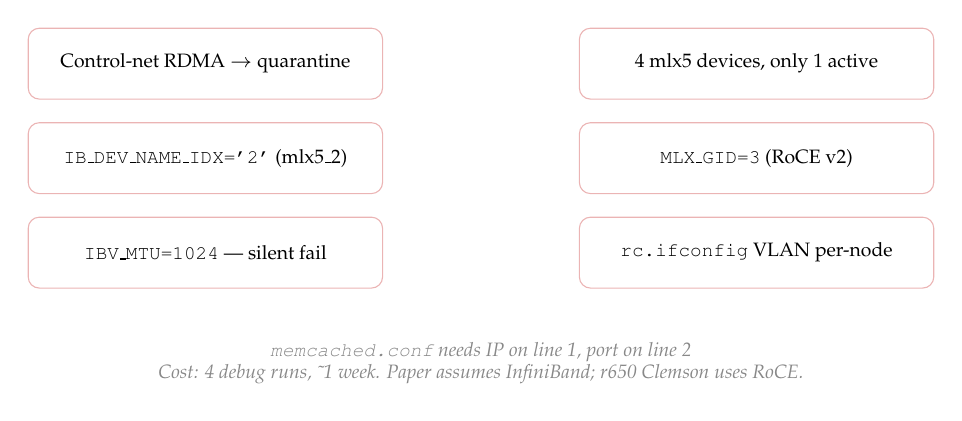
\begin{tikzpicture}[
  issue/.style={draw=mRed!40, rounded corners=4pt, minimum width=4.5cm,
                minimum height=0.9cm, align=center, font=\scriptsize},
]
  \node[issue] at (-3.5, 2.0) {Control-net RDMA $\to$ quarantine};
  \node[issue] at ( 3.5, 2.0) {4 mlx5 devices, only 1 active};
  \node[issue] at (-3.5, 0.8) {\texttt{IB\_DEV\_NAME\_IDX='2'} (mlx5\_2)};
  \node[issue] at ( 3.5, 0.8) {\texttt{MLX\_GID=3} (RoCE v2)};
  \node[issue] at (-3.5,-0.4) {\texttt{IBV\_MTU=1024} --- silent fail};
  \node[issue] at ( 3.5,-0.4) {\texttt{rc.ifconfig} VLAN per-node};
  \node[font=\scriptsize\itshape, mGray, align=center] at (0,-1.8)
    {\texttt{memcached.conf} needs IP on line 1, port on line 2\\
     Cost: 4 debug runs, \textasciitilde 1 week. Paper assumes InfiniBand; r650 Clemson uses RoCE.};
\end{tikzpicture}
\note{
  \textbf{Key point:} r650 Clemson uses RoCE, not InfiniBand. Six config
  changes needed before a single RDMA verb would fire.\\
  \textbf{Say:} The hardest part: r650 at Clemson uses RoCE---RDMA over
  Ethernet---not InfiniBand like the paper assumes. If you run RDMA on
  the control network CloudLab quarantines your account. The NIC exposes
  four mlx5 devices but only one is on the VLAN. We had to find the right
  device index, GID index, MTU, force VLAN bring-up per node, and debug
  an undocumented memcached config format. Four debug runs, about a week
  burned before we could run a single experiment.\\
  \textbf{Transition:} There was also a hard 16-hour wall.\\
  \textbf{Time:} 55s
}
\end{frame}

% Slide 16 — What Failed: The 16-Hour Wall
\begin{frame}{What Failed: The 16-Hour Wall}
\centering
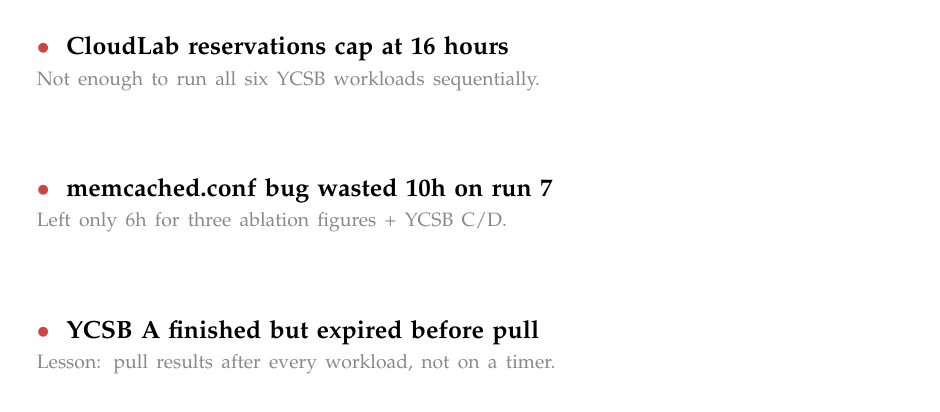
\begin{tikzpicture}[
  item/.style={font=\small, anchor=west, align=left, text width=11cm},
]
  \node[item] at (-5.5, 1.8)
    {{\color{mRed}$\bullet$}~~\textbf{CloudLab reservations cap at 16 hours}\\
     {\color{mGray}\scriptsize Not enough to run all six YCSB workloads sequentially.}};
  \node[item] at (-5.5, 0)
    {{\color{mRed}$\bullet$}~~\textbf{memcached.conf bug wasted 10h on run 7}\\
     {\color{mGray}\scriptsize Left only 6h for three ablation figures + YCSB C/D.}};
  \node[item] at (-5.5,-1.8)
    {{\color{mRed}$\bullet$}~~\textbf{YCSB A finished but expired before pull}\\
     {\color{mGray}\scriptsize Lesson: pull results after every workload, not on a timer.}};
\end{tikzpicture}
\note{
  \textbf{Key point:} The 16-hour reservation cap is the real bottleneck,
  not the code.\\
  \textbf{Say:} Even after RoCE was working, the 16-hour reservation cap
  was unforgiving. On run 7 a memcached.conf bug wasted 10 hours before
  I noticed, leaving only 6 hours for three figures. On run 8 YCSB A
  actually finished on the memory node but the reservation expired
  before I could pull the results. The lesson: pull results aggressively,
  after every workload, not on a timer.\\
  \textbf{Transition:} Why we failed where we did.\\
  \textbf{Time:} 45s
}
\end{frame}

% Slide 17 — Why We Failed
\begin{frame}{Why We Failed Where We Did}
\centering
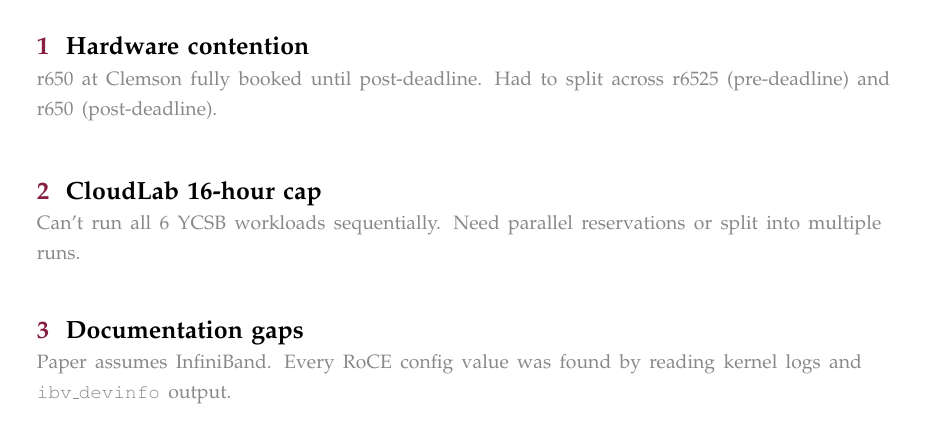
\begin{tikzpicture}[
  cause/.style={font=\small, anchor=west, align=left, text width=11cm},
]
  \node[cause] at (-5.5, 1.8)
    {{\color{mTeal}\textbf{1}}~~\textbf{Hardware contention}\\
     {\color{mGray}\scriptsize r650 at Clemson fully booked until post-deadline. Had to split across
                              r6525 (pre-deadline) and r650 (post-deadline).}};
  \node[cause] at (-5.5, 0)
    {{\color{mTeal}\textbf{2}}~~\textbf{CloudLab 16-hour cap}\\
     {\color{mGray}\scriptsize Can't run all 6 YCSB workloads sequentially. Need parallel reservations
                              or split into multiple runs.}};
  \node[cause] at (-5.5,-1.8)
    {{\color{mTeal}\textbf{3}}~~\textbf{Documentation gaps}\\
     {\color{mGray}\scriptsize Paper assumes InfiniBand. Every RoCE config value was found by reading
                              kernel logs and \texttt{ibv\_devinfo} output.}};
\end{tikzpicture}
\note{
  \textbf{Key point:} Three root causes, each with a fix for next time.\\
  \textbf{Say:} Three root causes. One, hardware contention---r650 at
  Clemson was booked solid so we had to split across two node types.
  Two, the 16-hour cap---six YCSB workloads just don't fit. Three,
  documentation---the paper assumes InfiniBand and every single RoCE
  config value had to be discovered by reading kernel logs. None of
  this is algorithmic---it's all infrastructure.\\
  \textbf{Transition:} That's Part One. Part Two is already underway.\\
  \textbf{Time:} 45s
}
\end{frame}

% Slide 18 — Next Steps: Part Two (CXL)
\begin{frame}{Next Steps: Part Two --- Porting CHIME to CXL}
\centering
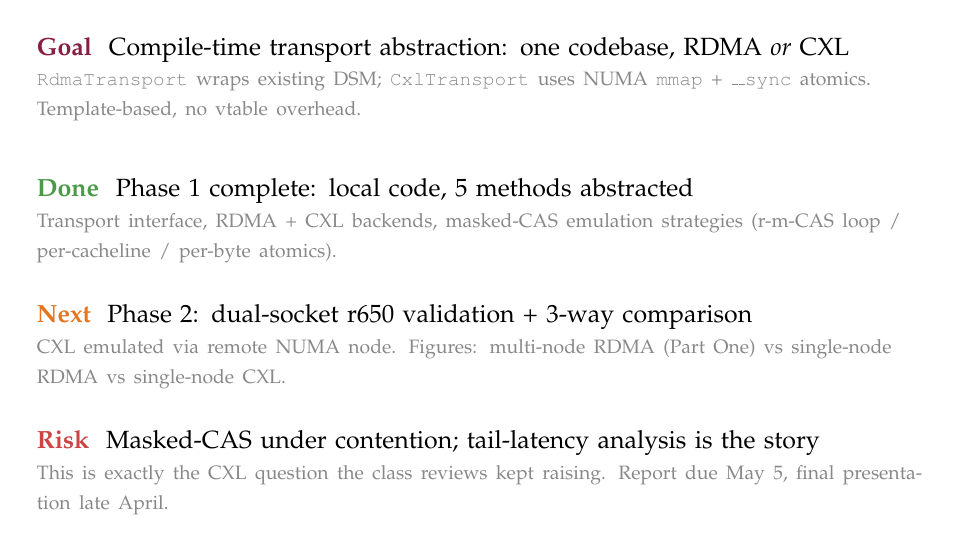
\begin{tikzpicture}[
  item/.style={font=\small, anchor=west, align=left, text width=11.5cm},
]
  \node[item] at (-5.8, 2.2)
    {{\color{mTeal}\textbf{Goal}}~~Compile-time transport abstraction: one codebase, RDMA \emph{or} CXL\\
     {\color{mGray}\scriptsize \texttt{RdmaTransport} wraps existing DSM; \texttt{CxlTransport} uses NUMA
                              \texttt{mmap} + \texttt{\_\_sync} atomics. Template-based, no vtable overhead.}};
  \node[item] at (-5.8, 0.4)
    {{\color{mGreen}\textbf{Done}}~~Phase 1 complete: local code, 5 methods abstracted\\
     {\color{mGray}\scriptsize Transport interface, RDMA + CXL backends, masked-CAS emulation
                              strategies (r-m-CAS loop / per-cacheline / per-byte atomics).}};
  \node[item] at (-5.8,-1.2)
    {{\color{mBrown}\textbf{Next}}~~Phase 2: dual-socket r650 validation + 3-way comparison\\
     {\color{mGray}\scriptsize CXL emulated via remote NUMA node. Figures: multi-node RDMA
                              (Part One) vs single-node RDMA vs single-node CXL.}};
  \node[item] at (-5.8,-2.8)
    {{\color{mRed}\textbf{Risk}}~~Masked-CAS under contention; tail-latency analysis is the story\\
     {\color{mGray}\scriptsize This is exactly the CXL question the class reviews kept raising.
                              Report due May 5, final presentation late April.}};
\end{tikzpicture}
\note{
  \textbf{Key point:} Transition to Part Two. The CXL port is already
  implemented at the code level; Phase 2 is cluster validation and the
  3-way comparison figures.\\
  \textbf{Say:} Before we go to discussion, quick update on Part Two.
  The goal is a clean transport abstraction: one codebase, either RDMA
  or CXL, chosen at compile time. No runtime overhead---templates, not
  virtual dispatch. Phase 1 is done---the transport interface is in,
  both RDMA and CXL backends are written, all five methods refactored
  to use it. CXL is emulated via NUMA on dual-socket r650. The
  interesting engineering challenge is masked-CAS emulation---there's
  no CPU equivalent, so I'm evaluating three strategies: a
  read-modify-CAS loop, per-cache-line locks, and per-byte atomics.
  Phase 2 is cluster validation and producing the three-way comparison:
  multi-node RDMA from Part One, single-node RDMA, and single-node CXL.
  And this is the exact question the class reviews kept raising---does
  CHIME's design survive under CXL? Report is due May 5.\\
  \textbf{Transition:} Which brings us to the discussion.\\
  \textbf{Time:} 75s
}
\end{frame}

% ============================================================
% SECTION 4: Discussion (11 slides, ~8 min)
% ============================================================

\section{Discussion}

% Slide 19 — Discussion divider (moved from end of deck)
{
\setbeamercolor{background canvas}{bg=myRed}
\begin{frame}[plain]
\vspace*{\fill}
\begin{center}
{\color{white}\Huge\bfseries Discussion}
\end{center}
\vspace*{\fill}
\note{
  \textbf{Key point:} Open floor transition.\\
  \textbf{Say:} That's the reproduction story. Now let's open it up---
  I've prepared specific prompts based on the class reviews, but any
  questions about the design or our experiments are welcome.\\
  \textbf{Transition:} Start with where the reviews converged.\\
  \textbf{Time:} 15s
}
\end{frame}
}

% Slide 20 — Reviewer Convergence
\begin{frame}{Where Reviewers Agreed}
\centering
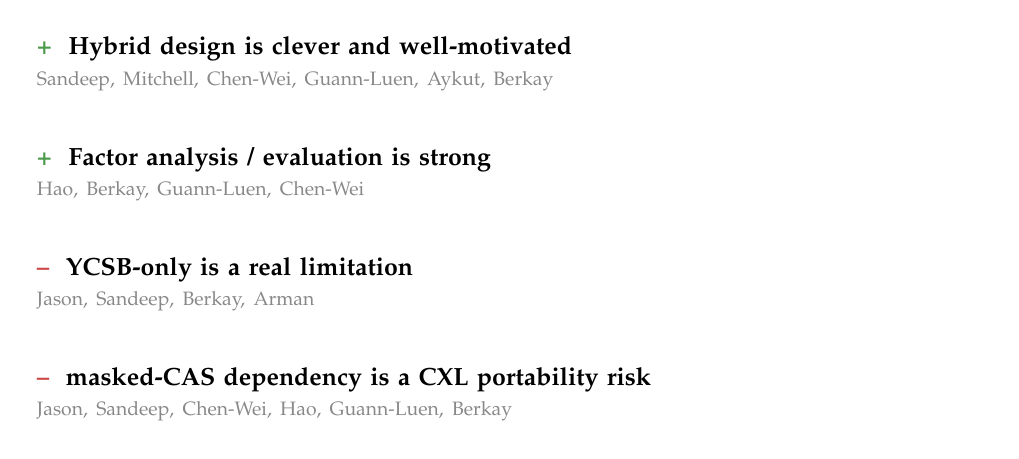
\begin{tikzpicture}[
  item/.style={font=\small, anchor=west, align=left, text width=12cm},
]
  \node[item] at (-6, 2.3)
    {{\color{mGreen}\textbf{+}}~~\textbf{Hybrid design is clever and well-motivated}\\
     {\color{mGray}\scriptsize Sandeep, Mitchell, Chen-Wei, Guann-Luen, Aykut, Berkay}};
  \node[item] at (-6, 0.9)
    {{\color{mGreen}\textbf{+}}~~\textbf{Factor analysis / evaluation is strong}\\
     {\color{mGray}\scriptsize Hao, Berkay, Guann-Luen, Chen-Wei}};
  \node[item] at (-6,-0.5)
    {{\color{mRed}\textbf{--}}~~\textbf{YCSB-only is a real limitation}\\
     {\color{mGray}\scriptsize Jason, Sandeep, Berkay, Arman}};
  \node[item] at (-6,-1.9)
    {{\color{mRed}\textbf{--}}~~\textbf{masked-CAS dependency is a CXL portability risk}\\
     {\color{mGray}\scriptsize Jason, Sandeep, Chen-Wei, Hao, Guann-Luen, Berkay}};
\end{tikzpicture}
\note{
  \textbf{Key point:} Four points of near-unanimous reviewer agreement:
  two positives (design + evaluation), two negatives (workloads + portability).\\
  \textbf{Say:} Before the specific prompts, here's where the reviews
  converged. Almost everyone agreed on four things. Two positives: the
  hybrid design is clever and well-motivated, and the factor analysis
  is unusually strong. Two negatives: YCSB-only is a real limitation,
  and the masked-CAS dependency puts CXL portability at risk. Six of
  the eleven reviews flagged the CXL issue specifically.\\
  \textbf{Transition:} And where they split.\\
  \textbf{Time:} 60s
}
\end{frame}

% Slide 21 — Reviewer Divergence
\begin{frame}{Where Reviewers Diverged}
\centering
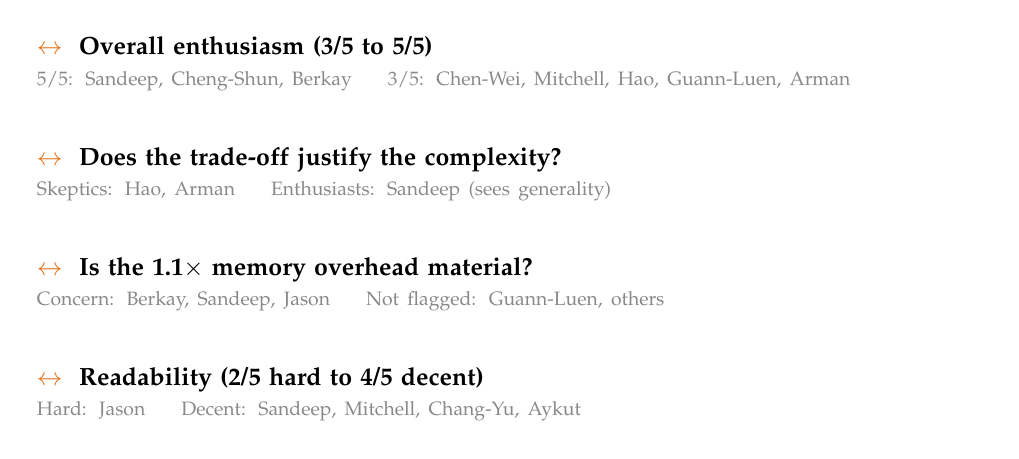
\begin{tikzpicture}[
  item/.style={font=\small, anchor=west, align=left, text width=12cm},
]
  \node[item] at (-6, 2.3)
    {{\color{mBrown}$\leftrightarrow$}~~\textbf{Overall enthusiasm (3/5 to 5/5)}\\
     {\color{mGray}\scriptsize 5/5: Sandeep, Cheng-Shun, Berkay \hspace{1em} 3/5: Chen-Wei, Mitchell, Hao, Guann-Luen, Arman}};
  \node[item] at (-6, 0.9)
    {{\color{mBrown}$\leftrightarrow$}~~\textbf{Does the trade-off justify the complexity?}\\
     {\color{mGray}\scriptsize Skeptics: Hao, Arman \hspace{1em} Enthusiasts: Sandeep (sees generality)}};
  \node[item] at (-6,-0.5)
    {{\color{mBrown}$\leftrightarrow$}~~\textbf{Is the 1.1$\times$ memory overhead material?}\\
     {\color{mGray}\scriptsize Concern: Berkay, Sandeep, Jason \hspace{1em} Not flagged: Guann-Luen, others}};
  \node[item] at (-6,-1.9)
    {{\color{mBrown}$\leftrightarrow$}~~\textbf{Readability (2/5 hard to 4/5 decent)}\\
     {\color{mGray}\scriptsize Hard: Jason \hspace{1em} Decent: Sandeep, Mitchell, Chang-Yu, Aykut}};
\end{tikzpicture}
\note{
  \textbf{Key point:} Four axes of disagreement. The interesting one is
  the complexity trade-off.\\
  \textbf{Say:} And here's where the reviews diverged. Enthusiasm ranged
  from 3 out of 5 all the way up to 5 out of 5---no one gave it lower
  than 3. The more interesting split is on complexity: Hao and Arman
  are skeptical that the gains justify the engineering cost, while
  Sandeep sees the techniques as broadly applicable and rated it 5/5.
  There's also a quiet disagreement about whether the 1.1x memory
  overhead is material, and a wide split on how hard the paper was
  to read.\\
  \textbf{Transition:} Let's dig into the specific prompts.\\
  \textbf{Time:} 60s
}
\end{frame}

% Slide 22 — Discussion: CXL Trade-off
\begin{frame}{Does the Trade-off Matter Under CXL?}
\centering
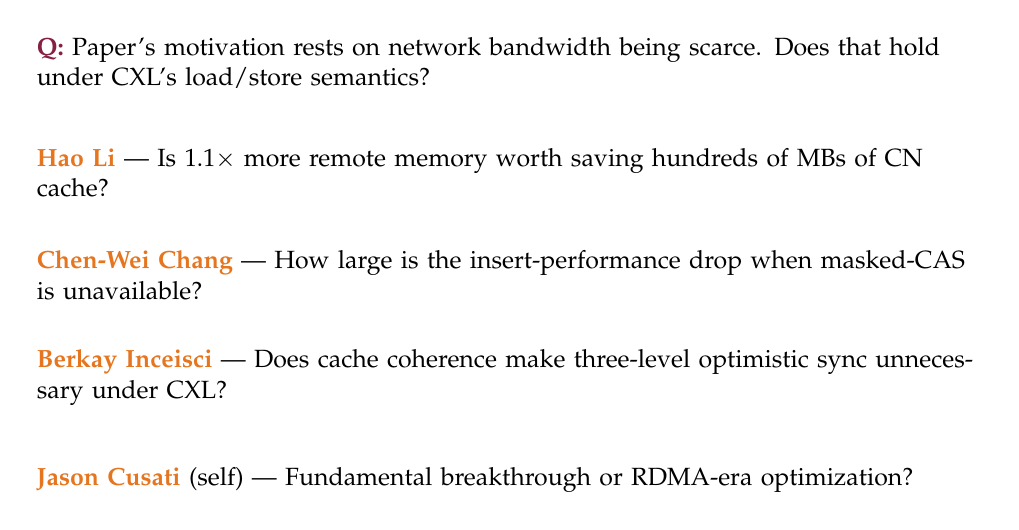
\begin{tikzpicture}[
  q/.style={font=\small, anchor=west, align=left, text width=12cm},
]
  \node[q] at (-6, 2.2)
    {{\color{mTeal}\textbf{Q:}} Paper's motivation rests on network bandwidth being scarce.
     Does that hold under CXL's load/store semantics?};
  \node[q] at (-6, 0.8)
    {{\color{mBrown}\textbf{Hao Li}} --- Is 1.1$\times$ more remote memory worth
     saving hundreds of MBs of CN cache?};
  \node[q] at (-6,-0.5)
    {{\color{mBrown}\textbf{Chen-Wei Chang}} --- How large is the insert-performance
     drop when masked-CAS is unavailable?};
  \node[q] at (-6,-1.8)
    {{\color{mBrown}\textbf{Berkay Inceisci}} --- Does cache coherence make
     three-level optimistic sync unnecessary under CXL?};
  \node[q] at (-6,-3.1)
    {{\color{mBrown}\textbf{Jason Cusati}} (self) --- Fundamental breakthrough
     or RDMA-era optimization?};
\end{tikzpicture}
\note{
  \textbf{Key point:} First discussion prompt. Names to call on: Hao Li,
  Chen-Wei Chang, Berkay Inceisci, myself (self-review).\\
  \textbf{Say:} First discussion question. The paper's whole motivation
  rests on network bandwidth being scarce and CN cache being precious.
  Does that hold under CXL? Hao, you flagged this in your review---is
  1.1 times more remote memory really worth saving hundreds of megs of
  cache on the compute nodes? Chen-Wei, you pointed out that the paper
  admits the piggybacking technique doesn't carry over to CXL but doesn't
  quantify the drop---how big do you think it would be? Berkay, you
  observed that CHIME uses only one-sided RDMA so it seems like a good
  CXL candidate, but the three-level sync might need revisiting under
  hardware cache coherence---which of those is the bigger blocker? And
  I raised it in my own review---is CHIME a fundamental breakthrough or
  an RDMA-era optimization that will age?\\
  \textbf{Transition:} Next---is the complexity worth it?\\
  \textbf{Time:} 75s
}
\end{frame}

% Slide 23 — Discussion: Complexity
\begin{frame}{Is the Complexity Worth It?}
\centering
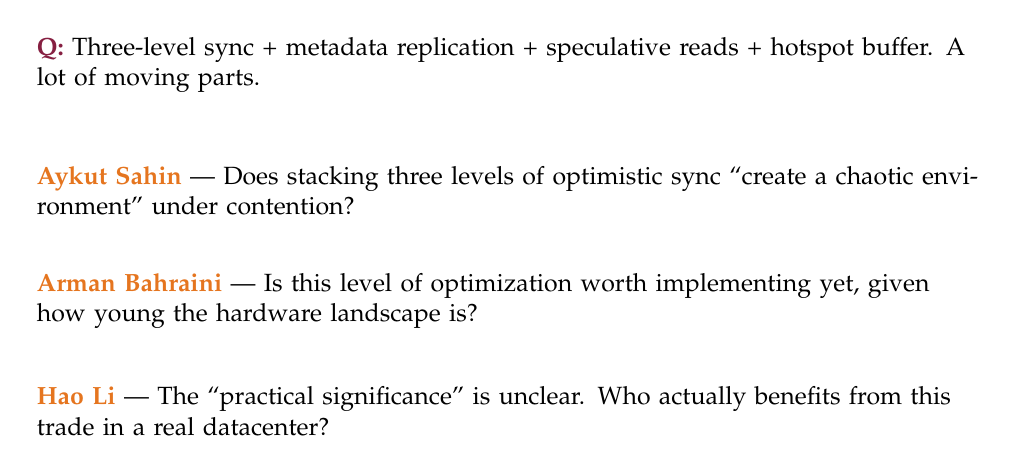
\begin{tikzpicture}[
  q/.style={font=\small, anchor=west, align=left, text width=12cm},
]
  \node[q] at (-6, 2.2)
    {{\color{mTeal}\textbf{Q:}} Three-level sync + metadata replication +
     speculative reads + hotspot buffer. A lot of moving parts.};
  \node[q] at (-6, 0.6)
    {{\color{mBrown}\textbf{Aykut Sahin}} --- Does stacking three levels of
     optimistic sync ``create a chaotic environment'' under contention?};
  \node[q] at (-6,-0.8)
    {{\color{mBrown}\textbf{Arman Bahraini}} --- Is this level of optimization
     worth implementing yet, given how young the hardware landscape is?};
  \node[q] at (-6,-2.2)
    {{\color{mBrown}\textbf{Hao Li}} --- The ``practical significance'' is
     unclear. Who actually benefits from this trade in a real datacenter?};
\end{tikzpicture}
\note{
  \textbf{Key point:} Second discussion prompt. Names: Aykut Sahin,
  Arman Bahraini, Hao Li.\\
  \textbf{Say:} Second question. CHIME stacks three separate sync levels,
  metadata replication, a speculative read path, and a hotspot buffer.
  Aykut, you flagged that stacking three levels of optimistic sync could
  create a chaotic environment under contention---do the factor analysis
  numbers convince you otherwise? Arman, you asked if this level of
  optimization is even worth implementing while the hardware landscape
  is still young. Where would you draw the line? And Hao, you wrote
  that the ``practical significance is less convincing''---who actually
  benefits from this trade in a real datacenter?\\
  \textbf{Transition:} Evaluation gaps next.\\
  \textbf{Time:} 75s
}
\end{frame}

% Slide 24 — Discussion: Evaluation Gaps
\begin{frame}{Evaluation Gaps}
\centering
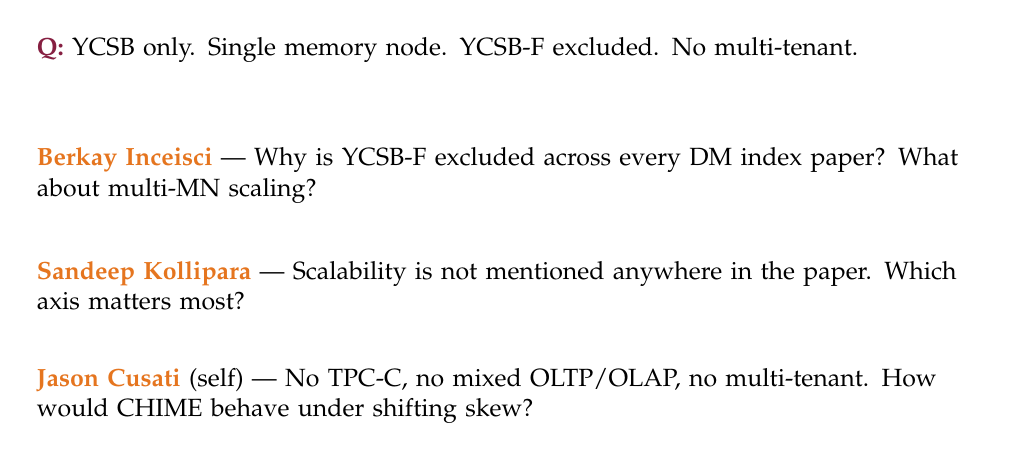
\begin{tikzpicture}[
  q/.style={font=\small, anchor=west, align=left, text width=12cm},
]
  \node[q] at (-6, 2.2)
    {{\color{mTeal}\textbf{Q:}} YCSB only. Single memory node. YCSB-F excluded.
     No multi-tenant.};
  \node[q] at (-6, 0.6)
    {{\color{mBrown}\textbf{Berkay Inceisci}} --- Why is YCSB-F excluded
     across every DM index paper? What about multi-MN scaling?};
  \node[q] at (-6,-0.8)
    {{\color{mBrown}\textbf{Sandeep Kollipara}} --- Scalability is not
     mentioned anywhere in the paper. Which axis matters most?};
  \node[q] at (-6,-2.2)
    {{\color{mBrown}\textbf{Jason Cusati}} (self) --- No TPC-C, no mixed
     OLTP/OLAP, no multi-tenant. How would CHIME behave under shifting skew?};
\end{tikzpicture}
\note{
  \textbf{Key point:} Third discussion prompt. Names: Berkay Inceisci,
  Sandeep Kollipara, self.\\
  \textbf{Say:} Third question---the evaluation. It's YCSB only, single
  memory node only. Berkay, you caught that YCSB-F is excluded across
  every DM index paper, not just this one. Any theory on why? And you
  asked about multi-memory-node scaling---does that matter for production?
  Sandeep, you noted that scalability isn't mentioned anywhere in the
  paper---what's the most important axis that went untested, compute
  nodes, memory nodes, or dataset size? And in my own review I flagged
  TPC-C, mixed OLTP/OLAP, and multi-tenant scenarios---how would
  CHIME behave when the skew actually shifts over time?\\
  \textbf{Transition:} But there's one specific workload where CHIME loses.\\
  \textbf{Time:} 75s
}
\end{frame}

% Slide 25 — Discussion: Range Scans (NEW)
\begin{frame}{Range Scans: Where ROLEX Wins}
\centering
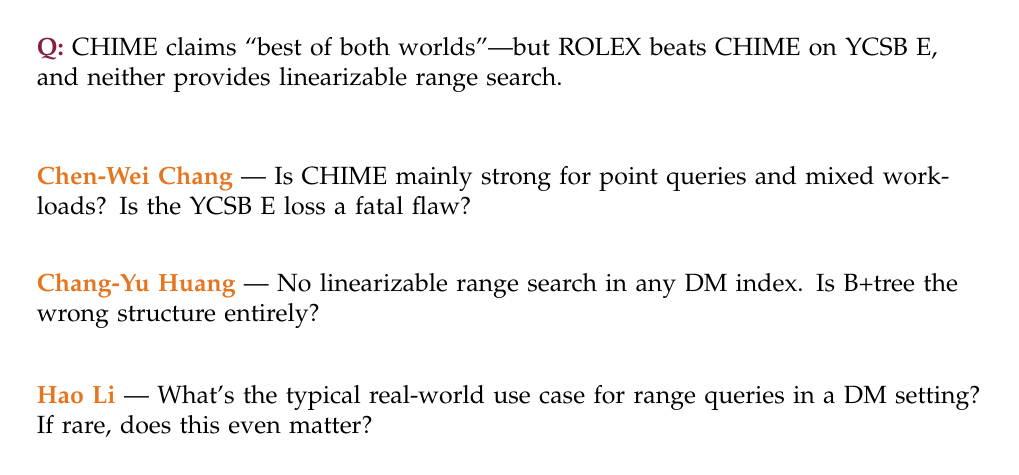
\begin{tikzpicture}[
  q/.style={font=\small, anchor=west, align=left, text width=12cm},
]
  \node[q] at (-6, 2.0)
    {{\color{mTeal}\textbf{Q:}} CHIME claims ``best of both worlds''---but ROLEX
     beats CHIME on YCSB E, and neither provides linearizable range search.};
  \node[q] at (-6, 0.4)
    {{\color{mBrown}\textbf{Chen-Wei Chang}} --- Is CHIME mainly strong for
     point queries and mixed workloads? Is the YCSB E loss a fatal flaw?};
  \node[q] at (-6,-1.0)
    {{\color{mBrown}\textbf{Chang-Yu Huang}} --- No linearizable range search
     in any DM index. Is B+tree the wrong structure entirely?};
  \node[q] at (-6,-2.4)
    {{\color{mBrown}\textbf{Hao Li}} --- What's the typical real-world use case
     for range queries in a DM setting? If rare, does this even matter?};
\end{tikzpicture}
\note{
  \textbf{Key point:} New discussion prompt on range scans.
  Names: Chen-Wei, Chang-Yu, Hao.\\
  \textbf{Say:} CHIME's whole pitch is breaking the range-vs-point
  trade-off, but ROLEX actually wins YCSB E---the scan-heavy workload.
  Chen-Wei, you wondered whether CHIME is mainly strong for point queries
  and mixed workloads rather than scan-heavy. Is that a fatal flaw for
  a range index? Chang-Yu, you raised a provocative point---neither
  CHIME nor Sherman provides linearizable range search, so maybe B+tree
  isn't the right structure for DM at all. What would replace it?
  And Hao, you asked the economic question: what's the typical real-world
  use case for range queries on DM? If they're rare, does losing on
  YCSB E even matter?\\
  \textbf{Transition:} The other gap---memory cost and failure handling.\\
  \textbf{Time:} 75s
}
\end{frame}

% Slide 26 — Discussion: Systems Gaps (NEW)
\begin{frame}{Systems Gaps: Memory Cost \& Failure Modes}
\centering
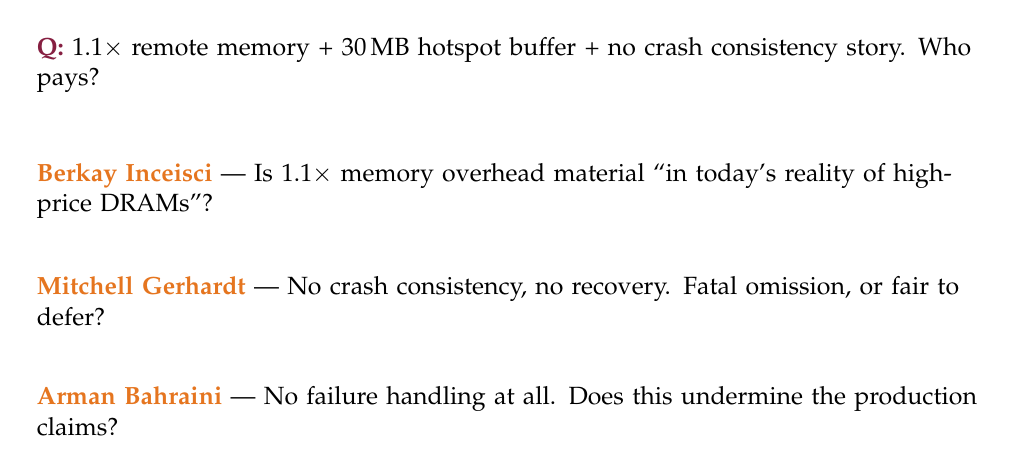
\begin{tikzpicture}[
  q/.style={font=\small, anchor=west, align=left, text width=12cm},
]
  \node[q] at (-6, 2.0)
    {{\color{mTeal}\textbf{Q:}} 1.1$\times$ remote memory + 30\,MB hotspot buffer +
     no crash consistency story. Who pays?};
  \node[q] at (-6, 0.4)
    {{\color{mBrown}\textbf{Berkay Inceisci}} --- Is 1.1$\times$ memory overhead
     material ``in today's reality of high-price DRAMs''?};
  \node[q] at (-6,-1.0)
    {{\color{mBrown}\textbf{Mitchell Gerhardt}} --- No crash consistency, no
     recovery. Fatal omission, or fair to defer?};
  \node[q] at (-6,-2.4)
    {{\color{mBrown}\textbf{Arman Bahraini}} --- No failure handling at all.
     Does this undermine the production claims?};
\end{tikzpicture}
\note{
  \textbf{Key point:} New discussion prompt on systems-level gaps:
  memory cost + failure handling. Names: Berkay, Mitchell, Arman.\\
  \textbf{Say:} Two overlapping gaps the paper doesn't address. On the
  memory side, CHIME adds 1.1 times remote memory overhead plus a 30 MB
  hotspot buffer on every compute node. Berkay, you flagged this as a
  real concern given today's DRAM prices---at what price point does the
  trade stop making sense? On the failure side, there's no crash
  consistency story, no recovery mechanism. Mitchell, is that a fatal
  omission for a SOSP paper, or fair to defer to follow-up work?
  Arman, you also flagged that CHIME doesn't delve into failure handling
  at all---does that undermine the production claims?\\
  \textbf{Transition:} A few detailed correctness concerns.\\
  \textbf{Time:} 75s
}
\end{frame}

% Slide 27 — Discussion: Design Details
\begin{frame}{Design Details Under Scrutiny}
\centering
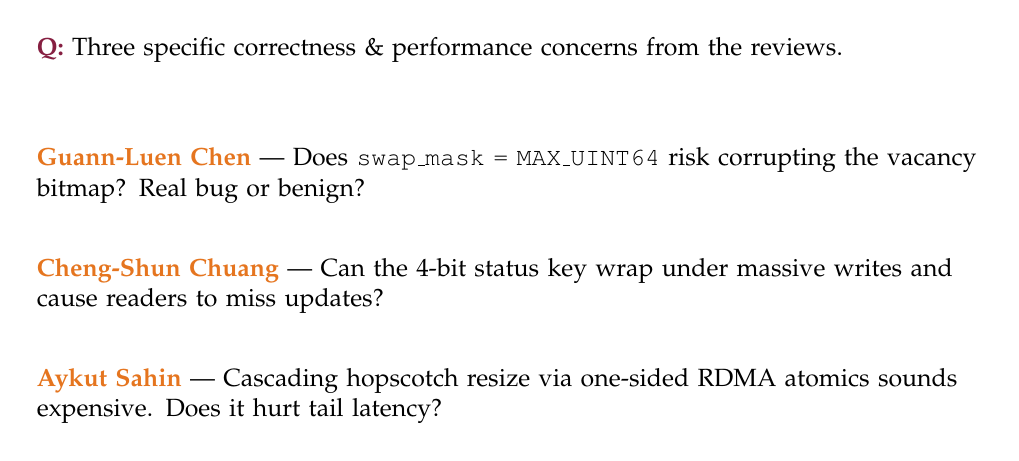
\begin{tikzpicture}[
  q/.style={font=\small, anchor=west, align=left, text width=12cm},
]
  \node[q] at (-6, 2.2)
    {{\color{mTeal}\textbf{Q:}} Three specific correctness \& performance concerns from the reviews.};
  \node[q] at (-6, 0.6)
    {{\color{mBrown}\textbf{Guann-Luen Chen}} --- Does \texttt{swap\_mask = MAX\_UINT64}
     risk corrupting the vacancy bitmap? Real bug or benign?};
  \node[q] at (-6,-0.8)
    {{\color{mBrown}\textbf{Cheng-Shun Chuang}} --- Can the 4-bit status key wrap
     under massive writes and cause readers to miss updates?};
  \node[q] at (-6,-2.2)
    {{\color{mBrown}\textbf{Aykut Sahin}} --- Cascading hopscotch resize via
     one-sided RDMA atomics sounds expensive. Does it hurt tail latency?};
\end{tikzpicture}
\note{
  \textbf{Key point:} Fourth discussion prompt. Names: Guann-Luen Chen,
  Cheng-Shun Chuang, Aykut Sahin.\\
  \textbf{Say:} Fourth question, for the detail-oriented. Guann-Luen, you
  had a specific technical concern about the vacancy bitmap piggybacking---
  the swap\_mask is set to all ones, which should overwrite the whole
  64-bit field including the bitmap. Is that a real bug, or did I miss
  something in the code? Cheng-Shun, you worried that the 4-bit status
  key could wrap around under extreme write contention and cause a reader
  to miss a concurrent update. Is 4 bits enough? And Aykut, you pointed
  out that hopscotch hashing is expensive to resize---cascading
  displacements via one-sided RDMA atomics sounds like a big penalty.
  Does that show up in tail latency under sustained insert workloads?\\
  \textbf{Transition:} Last discussion question---alternatives.\\
  \textbf{Time:} 75s
}
\end{frame}

% Slide 28 — Discussion: Alternatives
\begin{frame}{What Would You Build Instead?}
\centering
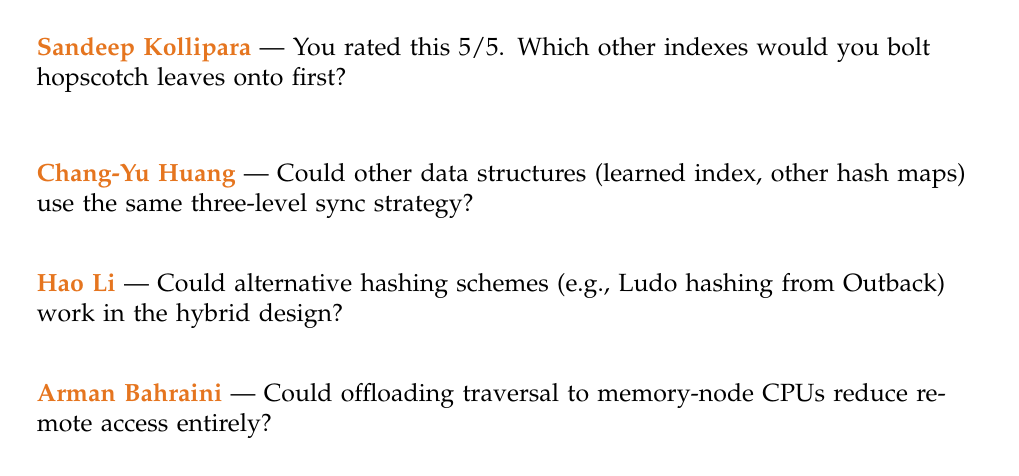
\begin{tikzpicture}[
  q/.style={font=\small, anchor=west, align=left, text width=12cm},
]
  \node[q] at (-6, 2.2)
    {{\color{mBrown}\textbf{Sandeep Kollipara}} --- You rated this 5/5.
     Which other indexes would you bolt hopscotch leaves onto first?};
  \node[q] at (-6, 0.6)
    {{\color{mBrown}\textbf{Chang-Yu Huang}} --- Could other data structures
     (learned index, other hash maps) use the same three-level sync strategy?};
  \node[q] at (-6,-0.8)
    {{\color{mBrown}\textbf{Hao Li}} --- Could alternative hashing schemes
     (e.g., Ludo hashing from Outback) work in the hybrid design?};
  \node[q] at (-6,-2.2)
    {{\color{mBrown}\textbf{Arman Bahraini}} --- Could offloading traversal
     to memory-node CPUs reduce remote access entirely?};
\end{tikzpicture}
\note{
  \textbf{Key point:} Fifth discussion prompt. Names: Sandeep Kollipara,
  Chang-Yu Huang, Hao Li, Arman Bahraini.\\
  \textbf{Say:} Last discussion question. Sandeep, you rated this 5 out
  of 5 and argued the hopscotch leaf is broadly applicable---which other
  indexes would you bolt it onto first? Chang-Yu, you also asked whether
  other data structures---learned indexes, other hash maps---could use
  the same three-level sync strategy. Is the sync the real reusable
  contribution, not the hybrid structure itself? Hao, you suggested
  alternative hashing schemes like Ludo hashing from Outback---what would
  change if we swapped hopscotch? And Arman, you raised the most
  provocative alternative: offload traversal to memory-node CPUs and
  reduce remote access entirely. Does that defeat disaggregation, or
  is it actually the right answer?\\
  \textbf{Transition:} Let me wrap up.\\
  \textbf{Time:} 75s
}
\end{frame}

% ============================================================
% SECTION 5: Close (2 slides, ~2 min)
% ============================================================

% Slide 29 — Key Takeaways
\begin{frame}{Key Takeaways}
\centering
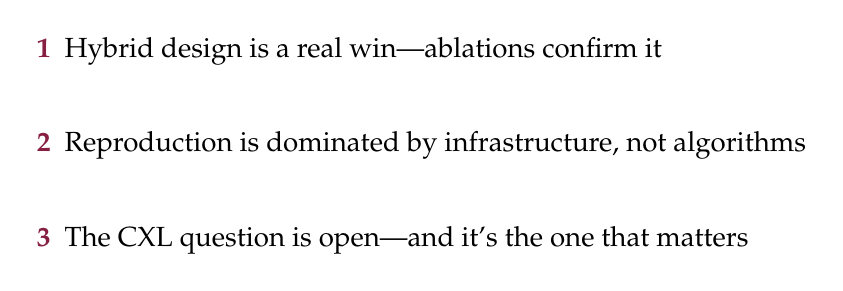
\begin{tikzpicture}[
  item/.style={font=\normalsize, anchor=west},
]
  \node[item] at (-4, 1.2) {{\color{mTeal}\textbf{1}}~~Hybrid design is a real win---ablations confirm it};
  \node[item] at (-4, 0)   {{\color{mTeal}\textbf{2}}~~Reproduction is dominated by infrastructure, not algorithms};
  \node[item] at (-4,-1.2) {{\color{mTeal}\textbf{3}}~~The CXL question is open---and it's the one that matters};
\end{tikzpicture}
\note{
  \textbf{Key point:} Three things to remember.\\
  \textbf{Say:} Three things to remember. First, CHIME's hybrid design
  is a real win---our r650 ablations confirm each technique contributes
  as claimed. Second, reproduction is dominated by infrastructure,
  not algorithms---80\% of our time was RoCE debugging, not CHIME.
  Third, the CXL question is the one that actually matters for whether
  this research ages well, and we'll answer it in Part Two.\\
  \textbf{Transition:} Thank you.\\
  \textbf{Time:} 40s
}
\end{frame}

% Slide 30 — References
\begin{frame}[allowframebreaks]{References}
\begin{thebibliography}{9}
\footnotesize

\bibitem{chime2024}
X.~Luo, J.~Shen, P.~Zuo, X.~Wang, M.~R.~Lyu, Y.~Zhou.
\newblock {CHIME}: A Cache-Efficient and High-Performance Hybrid Index on Disaggregated Memory.
\newblock \emph{SOSP}, 2024.

\bibitem{sherman2022}
Q.~Wang, Y.~Lu, J.~Shu.
\newblock {Sherman}: A Write-Optimized Distributed {B+Tree} Index on Disaggregated Memory.
\newblock \emph{SIGMETRICS}, 2022.

\bibitem{smart2023}
X.~Luo, P.~Zuo, J.~Shen, J.~Zhou, Y.~Zhou.
\newblock {SMART}: A High-Performance Adaptive Radix Tree for Disaggregated Memory.
\newblock \emph{USENIX ATC}, 2023.

\bibitem{rolex2024}
P.~Li, Y.~Hua, J.~Chen, J.~Zhang.
\newblock {ROLEX}: A Scalable {RDMA}-optimized Learned Key-Value Store for Disaggregated Memory Systems.
\newblock \emph{USENIX FAST}, 2023.

\bibitem{cxl}
CXL Consortium.
\newblock Compute Express Link Specification, Rev.~3.1.
\newblock 2024.

\end{thebibliography}
\note{
  \textbf{Key point:} Reference slide.\\
  \textbf{Say:} (No spoken content---reference slide for Q\&A.)\\
  \textbf{Transition:} ---\\
  \textbf{Time:} 5s
}
\end{frame}

\end{document}
